\chapter{Introduction}

\dfn{Database}{
    A \textit{Database} is defined as an organised collection of data that support on carrying out specific activities 
}

\section{Information system}

\dfn{Information system vs IT system}{
    A \textit{IS} is a structured combination of technology, people, and processes that handles piaces of information
}

Each IS supports pontentially other \textit{subsystems}, for this very reason it should be studied inside its operative context
\subsection{Handling the information}
Each IS handles the information within differenct aspects:
\begin{itemize}
    \item \textbf{Gathering / Acquisition}: collecting row data from different sources
    \begin{itemize}
        \item Gathering: collecting row data from different sources
        \item  Acquisition: capturing and importing data into the system
    \end{itemize}
    \item \textbf{Storing / Preservation}: Saving datas in a secure, organised way (for instance SQL table)
    \item \textbf{Elaboration / Transformation / Production}: processing row data into useful information
    \item \textbf{Distribution / Communication / Exchange}: making the processed information available to systems 
\end{itemize}

\nt{
    the idea of "IS" is independent from any computer automation. \\
    "Inforamtion system vs IT system!!!!"
}

note the following section:
\subsection{IT system}
\dfn{IT sys}{
    One of the aoutomated parts of the IS, in other words "It s the information system component that handle information using computer technologies"
}
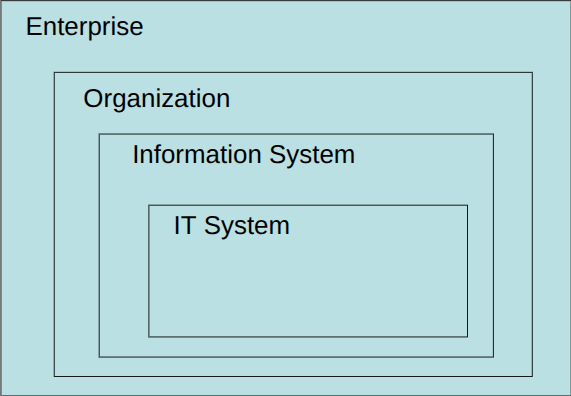
\includegraphics{imgs/itsys_vs_is.png}

\subsection{Information vs Data}
In IT sys, the \textit{Information} is expressed as \textit{data}. Look the differences:

\dfn{Inforamtion}{
    An \textit{information} is deifined as a facts or learned about something or someone
}
and
\dfn{Data}{
    A \textit{data} is defined pieces of information. A fixed starting point of a operation
}

\begin{quote}
these definitions are incorrects \\
\hfill --- Danilo
\end{quote}

\begin{quote}
F \\
\hfill --- Il Basta
\end{quote}

Data is simply the results of the process of orginising, coding and storing of information

\ex{Data vs information}{
    \begin{itemize}
        \item Infromation: "Mario Rossi, born in Rome, citizen ID 12345, lives at Via Roma 10"
        \item Data:
        \begin{tabular}{|c|c|c|c|}
            \hline
            Name & Surname & Tax Code & Address \\
            \hline
            Mario & Rossi & RSSMRA80A01H501X & Via Roma 10 \\
            \hline
        \end{tabular}

    \end{itemize}
}

TODO: BASTA PLEASE PROVIDE THE EXAMPLE!!! 

\subsubsection{Why Data}
First of all, handling information is difficult because the nature of information is often ambiguous. On the other hand, we use data because they are more stable and structured than other representations.

\section{Databses}
New definition, morespecific for icts:
\dfn{Database (for us)}{
    Set of data handled by a \textbf{DBMS}
}

% But... what tf is a DBMS? {\emojifont 🥀} sto emoji m

\subsection{Database management system (DBMS)}

\dfn{DBMS}{
    Any system handling data collections that are:
    \begin{itemize}
        \item big
        \item persistent
        \item shared: a db is an \textit{integrated} and \textit{shared} resources
    \end{itemize}
    ensuring
    \begin{itemize}
        \item privacy
        \item reliability
        \item efficiency
        \item effectivness
    \end{itemize}
}
\subsubsection{Problems}
\begin{itemize}
    \item Redundency: many repetiotions of a single data (nasty)
    \item 
\end{itemize}
